\documentclass{beamer}

%\usetheme{CambridgeUS}         % tema
% \usecolortheme{orchid}      % cores
\usetheme{metropolis}
\metroset{numbering=fraction, sectionpage=none, subsectionpage=progressbar}
\usecolortheme{seahorse}
\usecolortheme{rose}
\usefonttheme[onlysmall]{structurebold}
\usefonttheme[onlymath]{serif} % fonte modo matematico

\usepackage{framed}
\usepackage{disciplina}
\usepackage{tikz}
\usetikzlibrary{calc,shapes.multipart,chains,arrows}
\usepgflibrary{shapes.multipart}
\newcommand{\eq}{=}

\author[João Araujo Ribeiro]{João Araujo Ribeiro \\ \texttt{jaraujo@uerj.br}}
\institute[UERJ]{Universidade do Estado do Rio de Janeiro} % opcional
\date[EstrInf]{Departamento de Engenharia de Sistemas e Computação}
\pgfdeclareimage[height=0.7cm]{imagens//logo.png}{imagens//logodesc.png}
\logo{\pgfuseimage{imagens//logo.png}}
% Titulo
\title[\sc{Estruturas de Informação I}]{Estruturas de Informação I}
\subtitle{4. SkipLists}

\begin{document}

\begin{frame}
  \titlepage
\end{frame}

\begin{frame}
	\frametitle{Resumo}
	Nesta aula vamos estudar a skiplist.
	
	{\footnotesize \texttt{http://www.opendatastructures.org/ods-python/4\_Skiplists.html}}
	\tableofcontents
\end{frame}

\section{4 -  SkipList}

\subsection{4.1 Estrutura Básica}
\begin{frame}
	\LARGE{\alert{Estrutura Básica de uma SkipList}}
	
	\normalsize
	Conceitualmente, uma skiplist é uma sequência de listas encadeadas $ L_0,\ldots,L_h$. Cada lista $ L_r$ contém um subconjunto dos itens em $ L_{r-1}$. Começamos com a lista de entrada $ L_0$ que contém $ \ensuremath{\ensuremath{\mathit{n}}}$ itens e construímos $ L_1$ a partir de $ L_0$, $ L_2$ a partir de $ L_1$, e assim por diante. Os itens em $ L_r$ são obtidos pelo lançamento de uma moeda para cada elemento, $ \ensuremath{\ensuremath{\mathit{x}}}$, em $ L_{r-1}$ e incluindo $ \ensuremath{\ensuremath{\mathit{x}}}$ em $ L_r$ se a moeda dá cara. Este processo termina quando criamos uma lista vazia $ L_r$.
\end{frame}

\begin{frame}
\frametitle{Skiplist com 7 elementos}
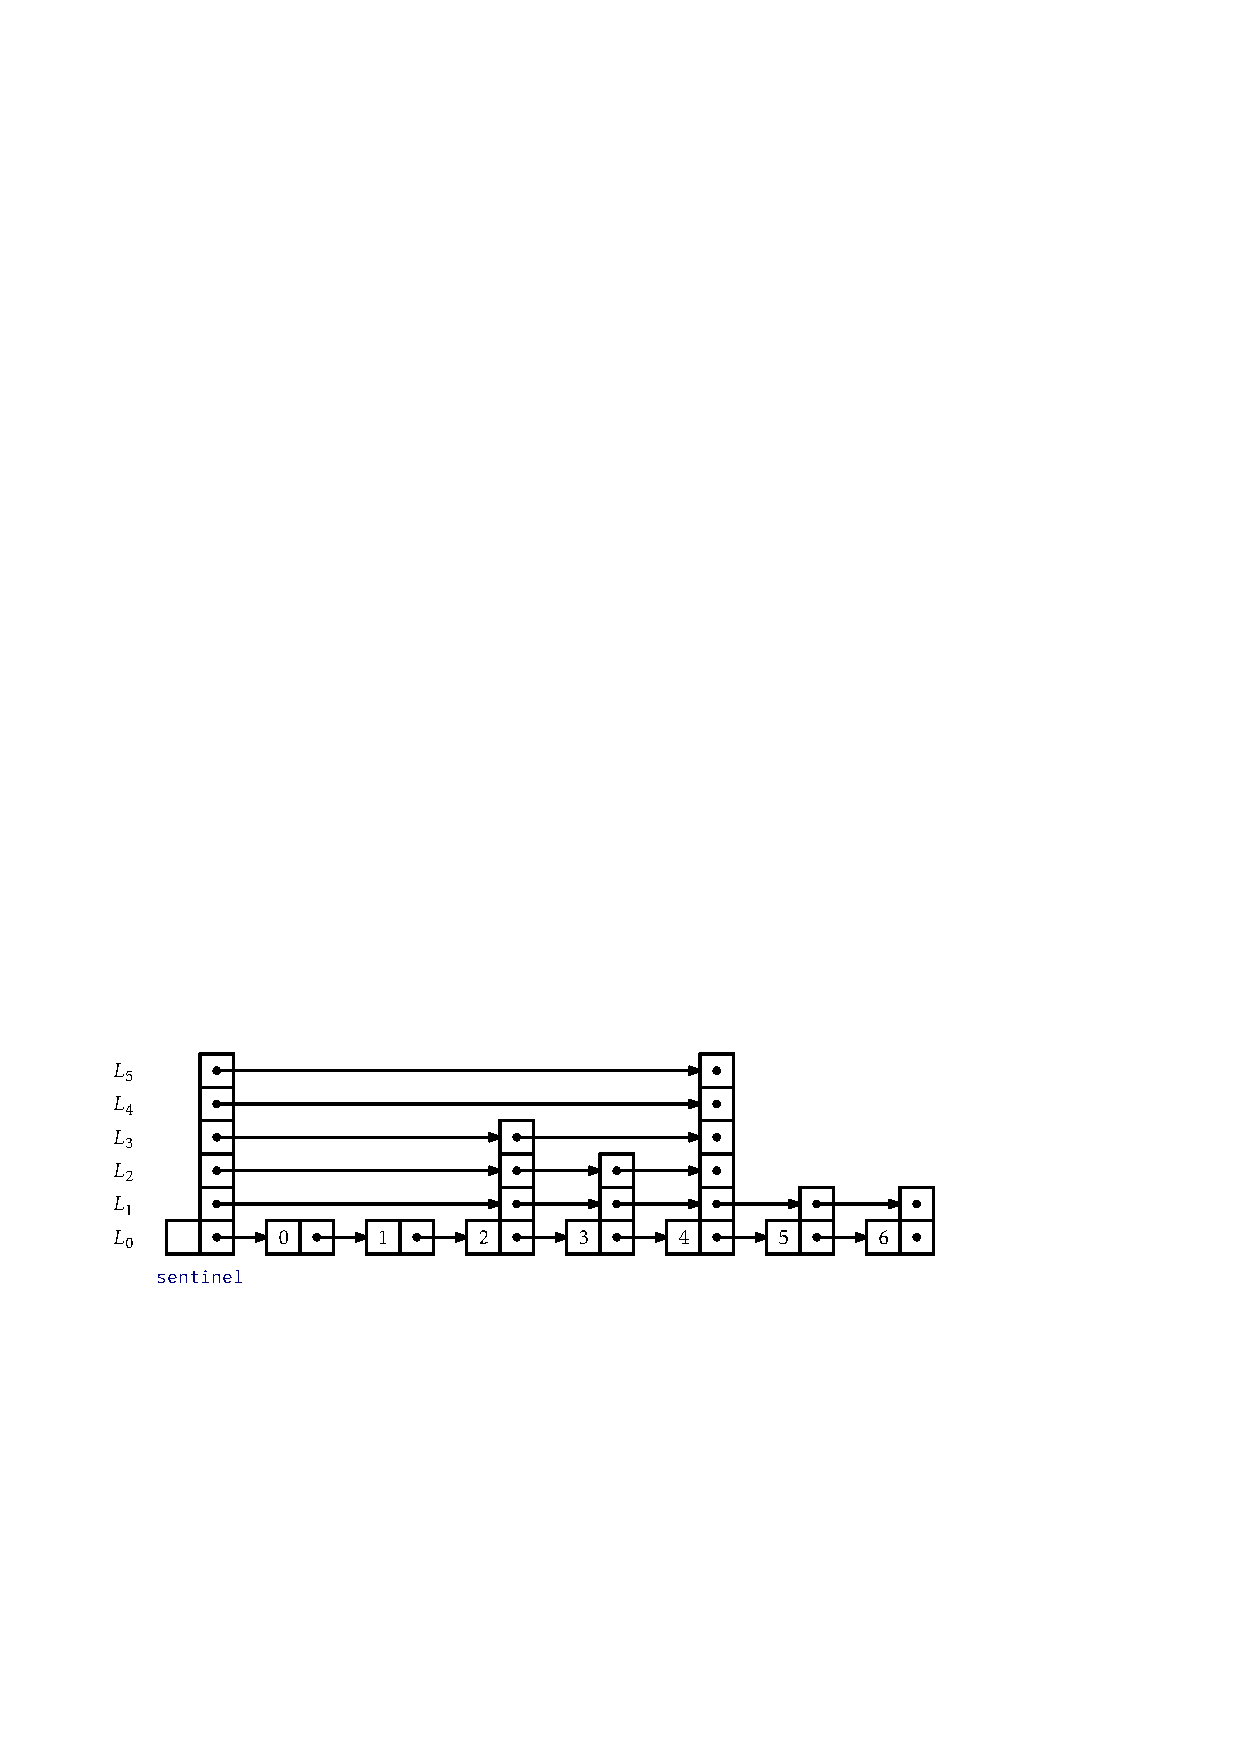
\includegraphics[scale=0.8]{imagens/skiplist}
\end{frame}

\begin{frame}
\frametitle{Altura de um elemento}
 A altura de um elemento $ \ensuremath{\ensuremath{\mathit{x}}}$, em uma \textit{skiplist}, é o valor mais alto de $ r$ tal que $ \ensuremath{\ensuremath{\mathit{x}}}$ apareça em $ L_r$. Assim, por exemplo, elementos que aparecem apenas em $ L_0$ têm altura 0.
\end{frame}




\begin{frame}
\frametitle{Caminho de busca}
Para construir um caminho de busca para o nó $ \ensuremath{\ensuremath{\mathit{u}}}$ em $ L_0$, começamos com o sentinela, $w$, em $L_h$. Depois, examinamos $ \ensuremath{\ensuremath{\mathit{w}}.\ensuremath{\mathit{next}}}$. Se $ \ensuremath{\ensuremath{\mathit{w}}.\ensuremath{\mathit{next}}}$ contém um item que aparece antes de $ \ensuremath{\ensuremath{\mathit{u}}}$ em $ L_0$, então fazemos $ \ensuremath{\ensuremath{\ensuremath{\mathit{w}}}}=\ensuremath{\ensuremath{\ensuremath{\mathit{w}}.\ensuremath{\mathit{next}}}}$. Caso contrário, nos movemos para baixo e continuamos a busca da ocorrência de  $ \ensuremath{\ensuremath{\mathit{w}}}$ na lista $ L_{h-1}$. Continuamos desta maneira até encontrarmos o predecessor de $ \ensuremath{\ensuremath{\mathit{u}}}$ em $ L_0$.  
\end{frame}

\begin{frame}
\frametitle{Caminho de busca para o nó contendo o valor 4}

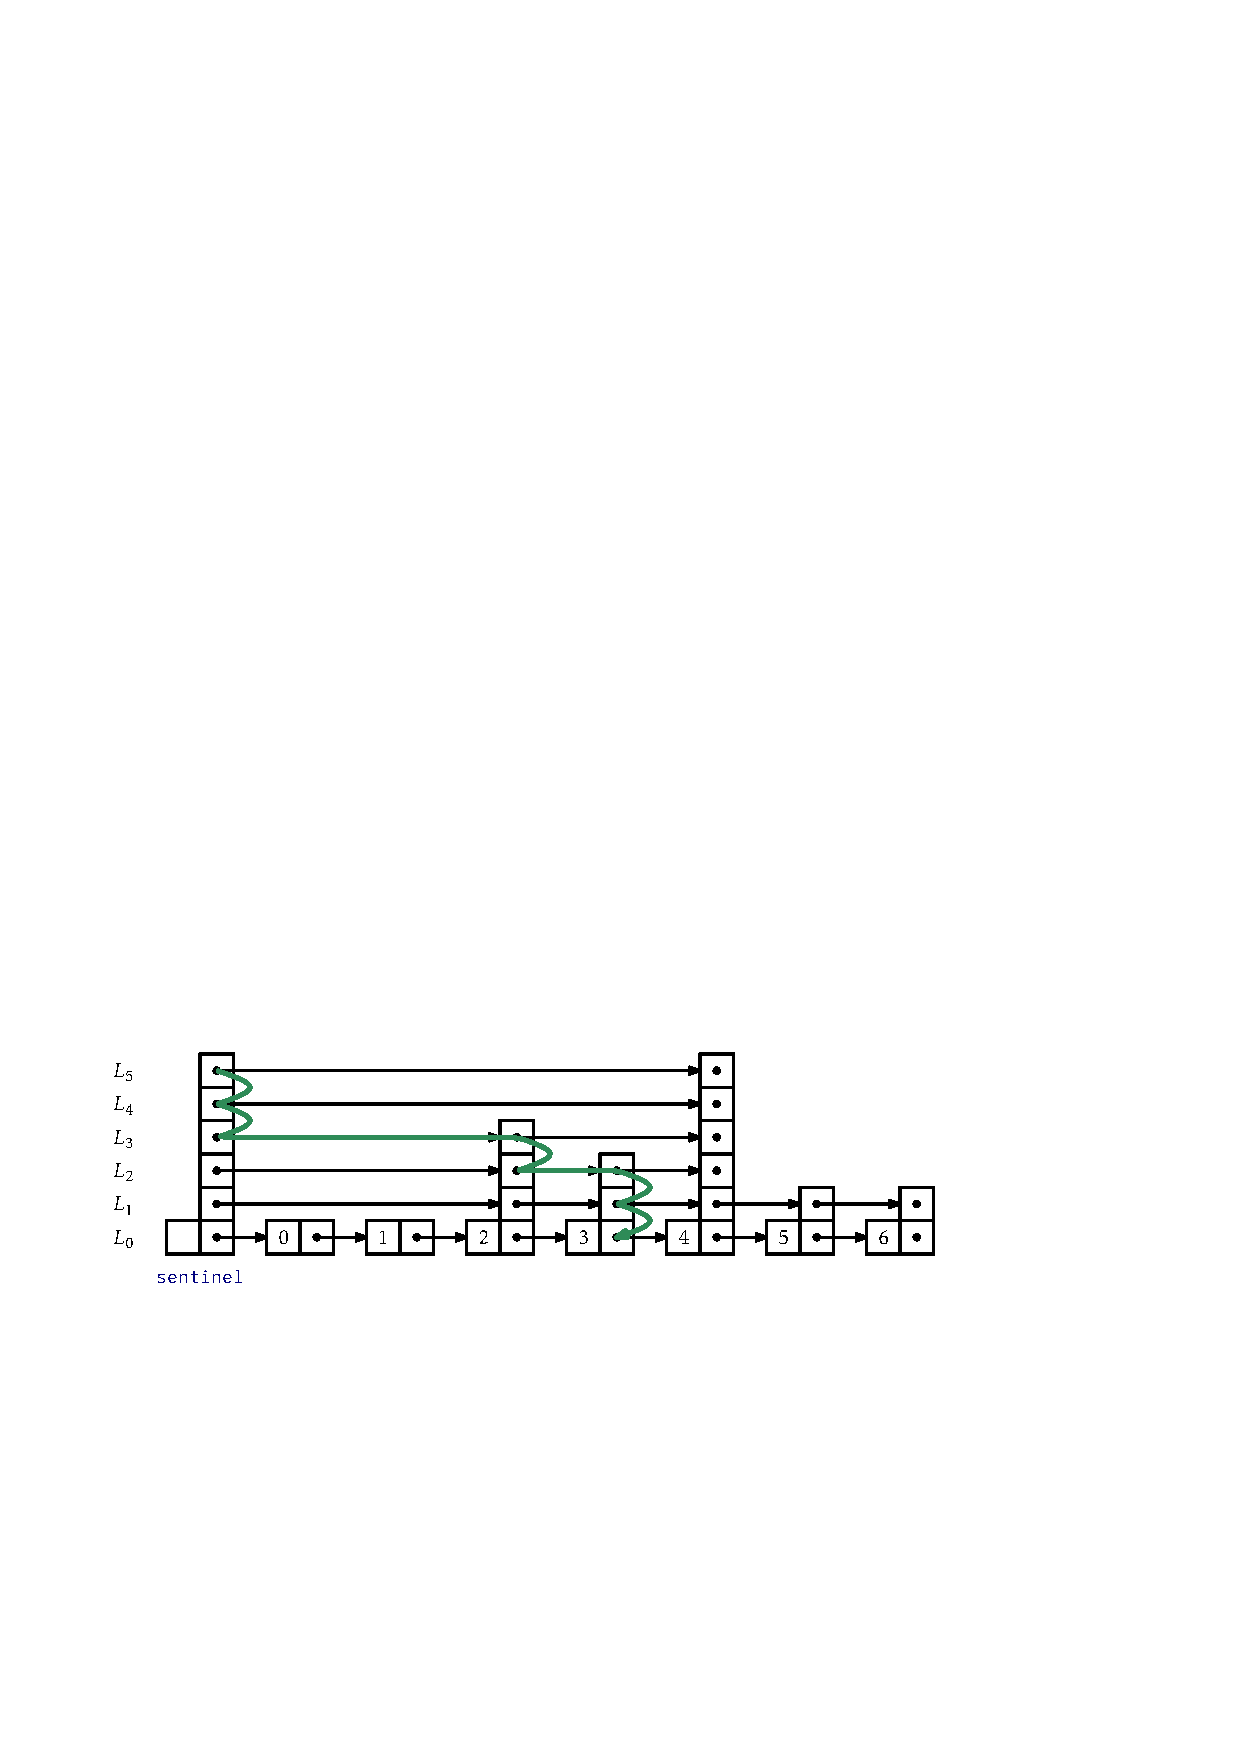
\includegraphics[scale=0.8]{imagens/skiplist-searchpath}

\end{frame}

\subsection{4.2 SkiplistSSet}
\begin{frame}
\frametitle{Uma implementação de um SSet com Skiplist}

Uma SkiplistSSet usa uma estrutura de skiplist para implementar a interface SSet.
\end{frame}

\begin{frame}[shrink]
\frametitle{$find(x)$}
\begin{oframed}
\begin{flushleft}
\ensuremath{\mathrm{find\_pred\_node}(\ensuremath{\mathit{x}})}\\
\hspace*{1em} \ensuremath{\ensuremath{\mathit{u}} \gets  \ensuremath{sentinel}}\\
\hspace*{1em} \ensuremath{\ensuremath{\mathit{r}} \gets  \ensuremath{h}}\\
\hspace*{1em} {\color{black} \textbf{while}} \ensuremath{\ensuremath{\mathit{r}} \ge 0} {\color{black} \textbf{do}} \\
\hspace*{1em} \hspace*{1em} {\color{black} \textbf{while}} \ensuremath{\ensuremath{\mathit{u}}.\ensuremath{\mathit{next}}[\ensuremath{\mathit{r}}] \ne nil} {\color{black} \textbf{and}} \ensuremath{\ensuremath{\mathit{u}}.\ensuremath{\mathit{next}}[\ensuremath{\mathit{r}}].\ensuremath{\mathit{x}} < x} {\color{black} \textbf{do}} \\
\hspace*{1em} \hspace*{1em} \hspace*{1em} \ensuremath{\ensuremath{\mathit{u}} \gets  \ensuremath{\ensuremath{\mathit{u}}.\ensuremath{\mathit{next}}[\ensuremath{\mathit{r}}]}  }\ {\color{blue}\# vai para direita na lista r}\\
\hspace*{1em} \hspace*{1em} \ensuremath{\ensuremath{\mathit{r}} \gets  \ensuremath{\ensuremath{\mathit{r}} - 1}  }\ {\color{blue}\# desce na lista r-1}\\
\hspace*{1em} {\color{black} \textbf{return}} \ensuremath{\ensuremath{\mathit{u}}}\\
\ \\
\ensuremath{\mathrm{find}(\ensuremath{\mathit{x}})}\\
\hspace*{1em} \ensuremath{\ensuremath{\mathit{u}} \gets  \ensuremath{\mathrm{find\_pred\_node}(\ensuremath{\mathit{x}})}}\\
\hspace*{1em} {\color{black} \textbf{if}} \ensuremath{\ensuremath{\mathit{u}}.\ensuremath{\mathit{next}}[0] \eq nil} {\color{black} \textbf{then}}  {\color{black} \textbf{return}} \ensuremath{\ensuremath{\mathit{nil}}}\\
\hspace*{1em} {\color{black} \textbf{return}} \ensuremath{\ensuremath{\mathit{u}}.\ensuremath{\mathit{next}}[0].\ensuremath{\mathit{x}}}\\
\end{flushleft}
\end{oframed}

\end{frame}

\begin{frame}
\frametitle{Simulando a jogada da moeda}
\begin{oframed}
\begin{flushleft}
\hspace*{1em} \ensuremath{\mathrm{pick\_height}()}\\
\hspace*{1em} \hspace*{1em} \ensuremath{\ensuremath{\mathit{z}} \gets  \ensuremath{\ensuremath{\mathit{random}}.\mathrm{getrandbits}(32)}}\\
\hspace*{1em} \hspace*{1em} \ensuremath{\ensuremath{\mathit{k}} \gets  \ensuremath{0}}\\
\hspace*{1em} \hspace*{1em} {\color{black} \textbf{while}} \ensuremath{\ensuremath{\mathit{z}}  \wedge  1} {\color{black} \textbf{do}} \\
\hspace*{1em} \hspace*{1em} \hspace*{1em} \ensuremath{\ensuremath{\mathit{k}} \gets  \ensuremath{\ensuremath{\mathit{k}} + 1}}\\
\hspace*{1em} \hspace*{1em} \hspace*{1em} \ensuremath{\ensuremath{\mathit{z}} \gets  \ensuremath{\ensuremath{\mathit{z}}}} div  $2$\\
\hspace*{1em} \hspace*{1em} {\color{black} \textbf{return}} \ensuremath{\ensuremath{\mathit{k}}}\\
\end{flushleft}
\end{oframed}
\end{frame}

\begin{frame}[shrink]
\frametitle{$add(x)$}
\begin{flushleft}
\ensuremath{\mathrm{add}(\ensuremath{\mathit{x}})}\\
\hspace*{1em} \ensuremath{\ensuremath{\mathit{u}} \gets  \ensuremath{sentinel}}\\
\hspace*{1em} \ensuremath{\ensuremath{\mathit{r}} \gets  \ensuremath{h}}\\
\hspace*{1em} {\color{black} \textbf{while}} \ensuremath{\ensuremath{\mathit{r}} \ge 0} {\color{black} \textbf{do}} \\
\hspace*{1em} \hspace*{1em} {\color{black} \textbf{while}} \ensuremath{\ensuremath{\mathit{u}}.\ensuremath{\mathit{next}}[\ensuremath{\mathit{r}}] \ne nil} {\color{black} \textbf{and}} \ensuremath{\ensuremath{\mathit{u}}.\ensuremath{\mathit{next}}[\ensuremath{\mathit{r}}].\ensuremath{\mathit{x}} < x} {\color{black} \textbf{do}} \\
\hspace*{1em} \hspace*{1em} \hspace*{1em} \ensuremath{\ensuremath{\mathit{u}} \gets  \ensuremath{\ensuremath{\mathit{u}}.\ensuremath{\mathit{next}}[\ensuremath{\mathit{r}}]}}\\
\hspace*{1em} \hspace*{1em} {\color{black} \textbf{if}} \ensuremath{\ensuremath{\mathit{u}}.\ensuremath{\mathit{next}}[\ensuremath{\mathit{r}}] \ne nil} {\color{black} \textbf{and}} \ensuremath{\ensuremath{\mathit{u}}.\ensuremath{\mathit{next}}[\ensuremath{\mathit{r}}].\ensuremath{\mathit{x}} \eq x} {\color{black} \textbf{then}}\\
\hspace*{1em} \hspace*{1em} \hspace*{1em}   {\color{black} \textbf{return}} \ensuremath{\ensuremath{\mathit{false}}}\\
\hspace*{1em} \hspace*{1em} \ensuremath{\ensuremath{\mathit{stack}}[\ensuremath{r}] \gets  \ensuremath{u}}\\
\hspace*{1em} \hspace*{1em} \ensuremath{\ensuremath{\mathit{r}} \gets  \ensuremath{\ensuremath{\mathit{r}} - 1}}\\
\hspace*{1em} \ensuremath{\ensuremath{\mathit{w}} \gets  \ensuremath{\mathrm{new\_node}(\ensuremath{\mathit{x}}, \mathrm{pick\_height}()})}\\
\hspace*{1em} {\color{black} \textbf{while}} \ensuremath{\ensuremath{\mathit{h}} < \ensuremath{\mathit{w}}.\mathrm{height}()} {\color{black} \textbf{do}} \\
\hspace*{1em} \hspace*{1em} \ensuremath{\ensuremath{\mathit{h}} \gets  \ensuremath{\ensuremath{\mathit{h}} + 1}}\\
\hspace*{1em} \hspace*{1em} \ensuremath{\ensuremath{\mathit{stack}}[\ensuremath{h}] \gets  \ensuremath{sentinel}   }\ {\color{blue}\# altura aumentada}\\
\hspace*{1em} {\color{black} \textbf{for}} \ensuremath{i} {\color{black} \textbf{in}} \ensuremath{0,1,2,\ldots,\mathrm{len}(\ensuremath{\mathit{w}}.\ensuremath{\mathit{next}})-1} {\color{black} \textbf{do}} \\
\hspace*{1em} \hspace*{1em} \ensuremath{\ensuremath{\mathit{w}}.\ensuremath{\ensuremath{\mathit{next}}[\ensuremath{\mathit{i}}]} \gets  \ensuremath{\ensuremath{\mathit{stack}}[\ensuremath{\mathit{i}}].\ensuremath{\mathit{next}}[\ensuremath{\mathit{i}}]}}\\
\hspace*{1em} \hspace*{1em} \ensuremath{\ensuremath{\mathit{stack}}[\ensuremath{i}].\ensuremath{\ensuremath{\mathit{next}}[\ensuremath{\mathit{i}}]} \gets  \ensuremath{w}}\\
\hspace*{1em} \ensuremath{\ensuremath{\mathit{n}} \gets  \ensuremath{\ensuremath{\mathit{n}} + 1}}\\
\hspace*{1em} {\color{black} \textbf{return}} \ensuremath{\ensuremath{\mathit{true}}}\\
\end{flushleft}

\end{frame}

\begin{frame}
\frametitle{$add(3.5)$}
Os nós de $stack$ estão coloridos.
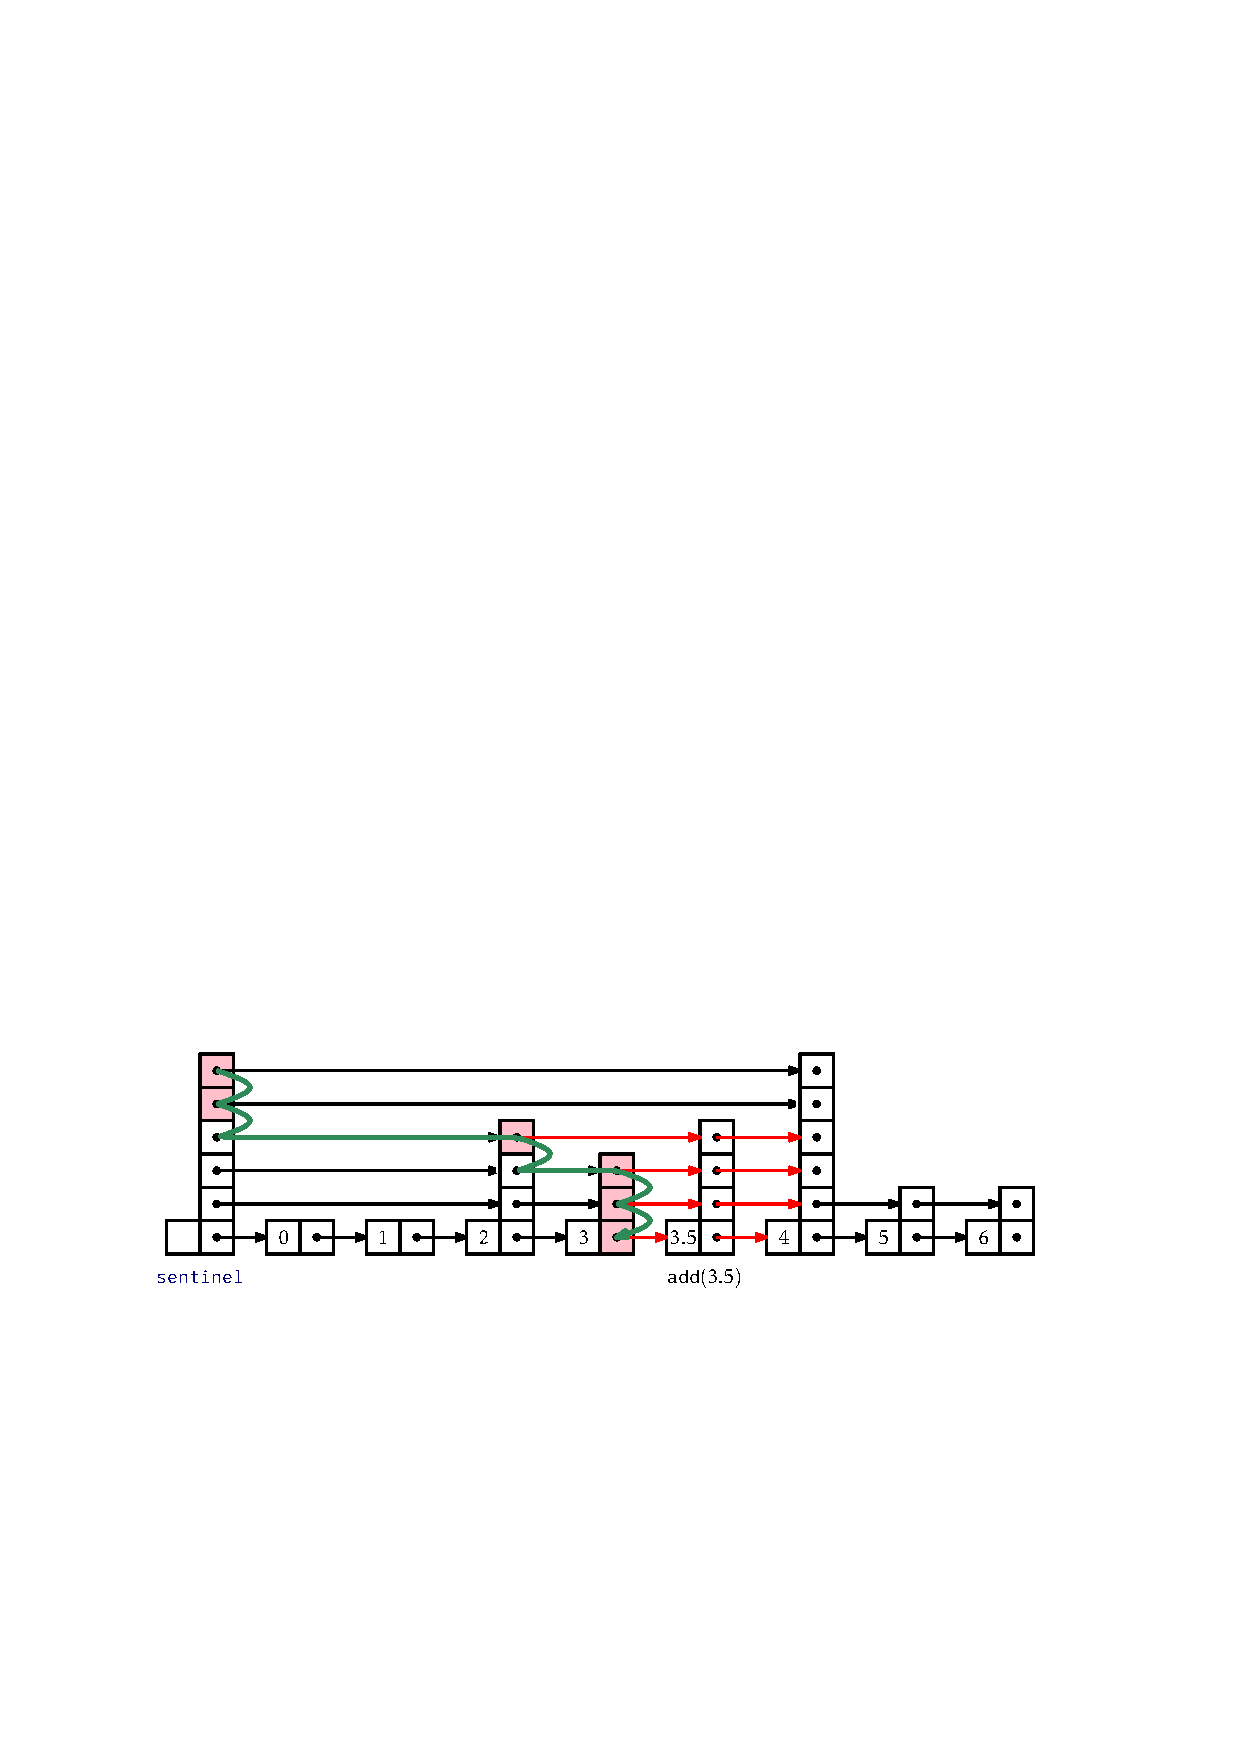
\includegraphics[scale=0.75]{imagens/skiplist-add}
\end{frame}

\begin{frame}[shrink]
\frametitle{$remove(x)$}
\begin{oframed}
\begin{flushleft}
\hspace*{1em} \ensuremath{\mathrm{remove}(\ensuremath{\mathit{x}})}\\
\hspace*{1em} \hspace*{1em} \ensuremath{\ensuremath{\mathit{removed}} \gets  \ensuremath{\ensuremath{\mathit{false}}}}\\
\hspace*{1em} \hspace*{1em} \ensuremath{\ensuremath{\mathit{u}} \gets  \ensuremath{sentinel}}\\
\hspace*{1em} \hspace*{1em} \ensuremath{\ensuremath{\mathit{r}} \gets  \ensuremath{h}}\\
\hspace*{1em} \hspace*{1em} {\color{black} \textbf{while}} \ensuremath{\ensuremath{\mathit{r}} \ge 0} {\color{black} \textbf{do}} \\
\hspace*{1em} \hspace*{1em} \hspace*{1em} {\color{black} \textbf{while}} \ensuremath{\ensuremath{\mathit{u}}.\ensuremath{\mathit{next}}[\ensuremath{\mathit{r}}] \ne nil} {\color{black} \textbf{and}} \ensuremath{\ensuremath{\mathit{u}}.\ensuremath{\mathit{next}}[\ensuremath{\mathit{r}}].\ensuremath{\mathit{x}} < x} {\color{black} \textbf{do}} \\
\hspace*{1em} \hspace*{1em} \hspace*{1em} \hspace*{1em} \ensuremath{\ensuremath{\mathit{u}} \gets  \ensuremath{\ensuremath{\mathit{u}}.\ensuremath{\mathit{next}}[\ensuremath{\mathit{r}}]}}\\
\hspace*{1em} \hspace*{1em} \hspace*{1em} {\color{black} \textbf{if}} \ensuremath{\ensuremath{\mathit{u}}.\ensuremath{\mathit{next}}[\ensuremath{\mathit{r}}] \ne nil} {\color{black} \textbf{and}} \ensuremath{\ensuremath{\mathit{u}}.\ensuremath{\mathit{next}}[\ensuremath{\mathit{r}}].\ensuremath{\mathit{x}} \eq x} {\color{black} \textbf{then}} \\
\hspace*{1em} \hspace*{1em} \hspace*{1em} \hspace*{1em} \ensuremath{\ensuremath{\mathit{removed}} \gets  \ensuremath{\ensuremath{\mathit{true}}}}\\
\hspace*{1em} \hspace*{1em} \hspace*{1em} \hspace*{1em} \ensuremath{\ensuremath{\mathit{u}}.\ensuremath{\ensuremath{\mathit{next}}[\ensuremath{\mathit{r}}]} \gets  \ensuremath{\ensuremath{\mathit{u}}.\ensuremath{\mathit{next}}[\ensuremath{\mathit{r}}].\ensuremath{\mathit{next}}[\ensuremath{\mathit{r}}]}}\\
\hspace*{1em} \hspace*{1em} \hspace*{1em} \hspace*{1em} {\color{black} \textbf{if}} \ensuremath{\ensuremath{\mathit{u}} \eq sentinel} {\color{black} \textbf{and}} \ensuremath{\ensuremath{\mathit{u}}.\ensuremath{\mathit{next}}[\ensuremath{\mathit{r}}] \eq nil} {\color{black} \textbf{then}} \\
\hspace*{1em} \hspace*{1em} \hspace*{1em} \hspace*{1em} \hspace*{1em} \ensuremath{\ensuremath{\mathit{h}} \gets  \ensuremath{\ensuremath{\mathit{h}} - 1} }\ {\color{blue}\# altura foi diminuída}\\
\hspace*{1em} \hspace*{1em} \hspace*{1em} \ensuremath{\ensuremath{\mathit{r}} \gets  \ensuremath{\ensuremath{\mathit{r}} - 1}}\\
\hspace*{1em} \hspace*{1em} {\color{black} \textbf{if}} \ensuremath{removed} {\color{black} \textbf{then}}  \ensuremath{\ensuremath{\mathit{n}} \gets  \ensuremath{\ensuremath{\mathit{n}} - 1}}\\
\hspace*{1em} \hspace*{1em} {\color{black} \textbf{return}} \ensuremath{removed}\hspace*{1em} \\
\end{flushleft}
\end{oframed}
\end{frame}

\begin{frame}
\frametitle{$remove(3)$}
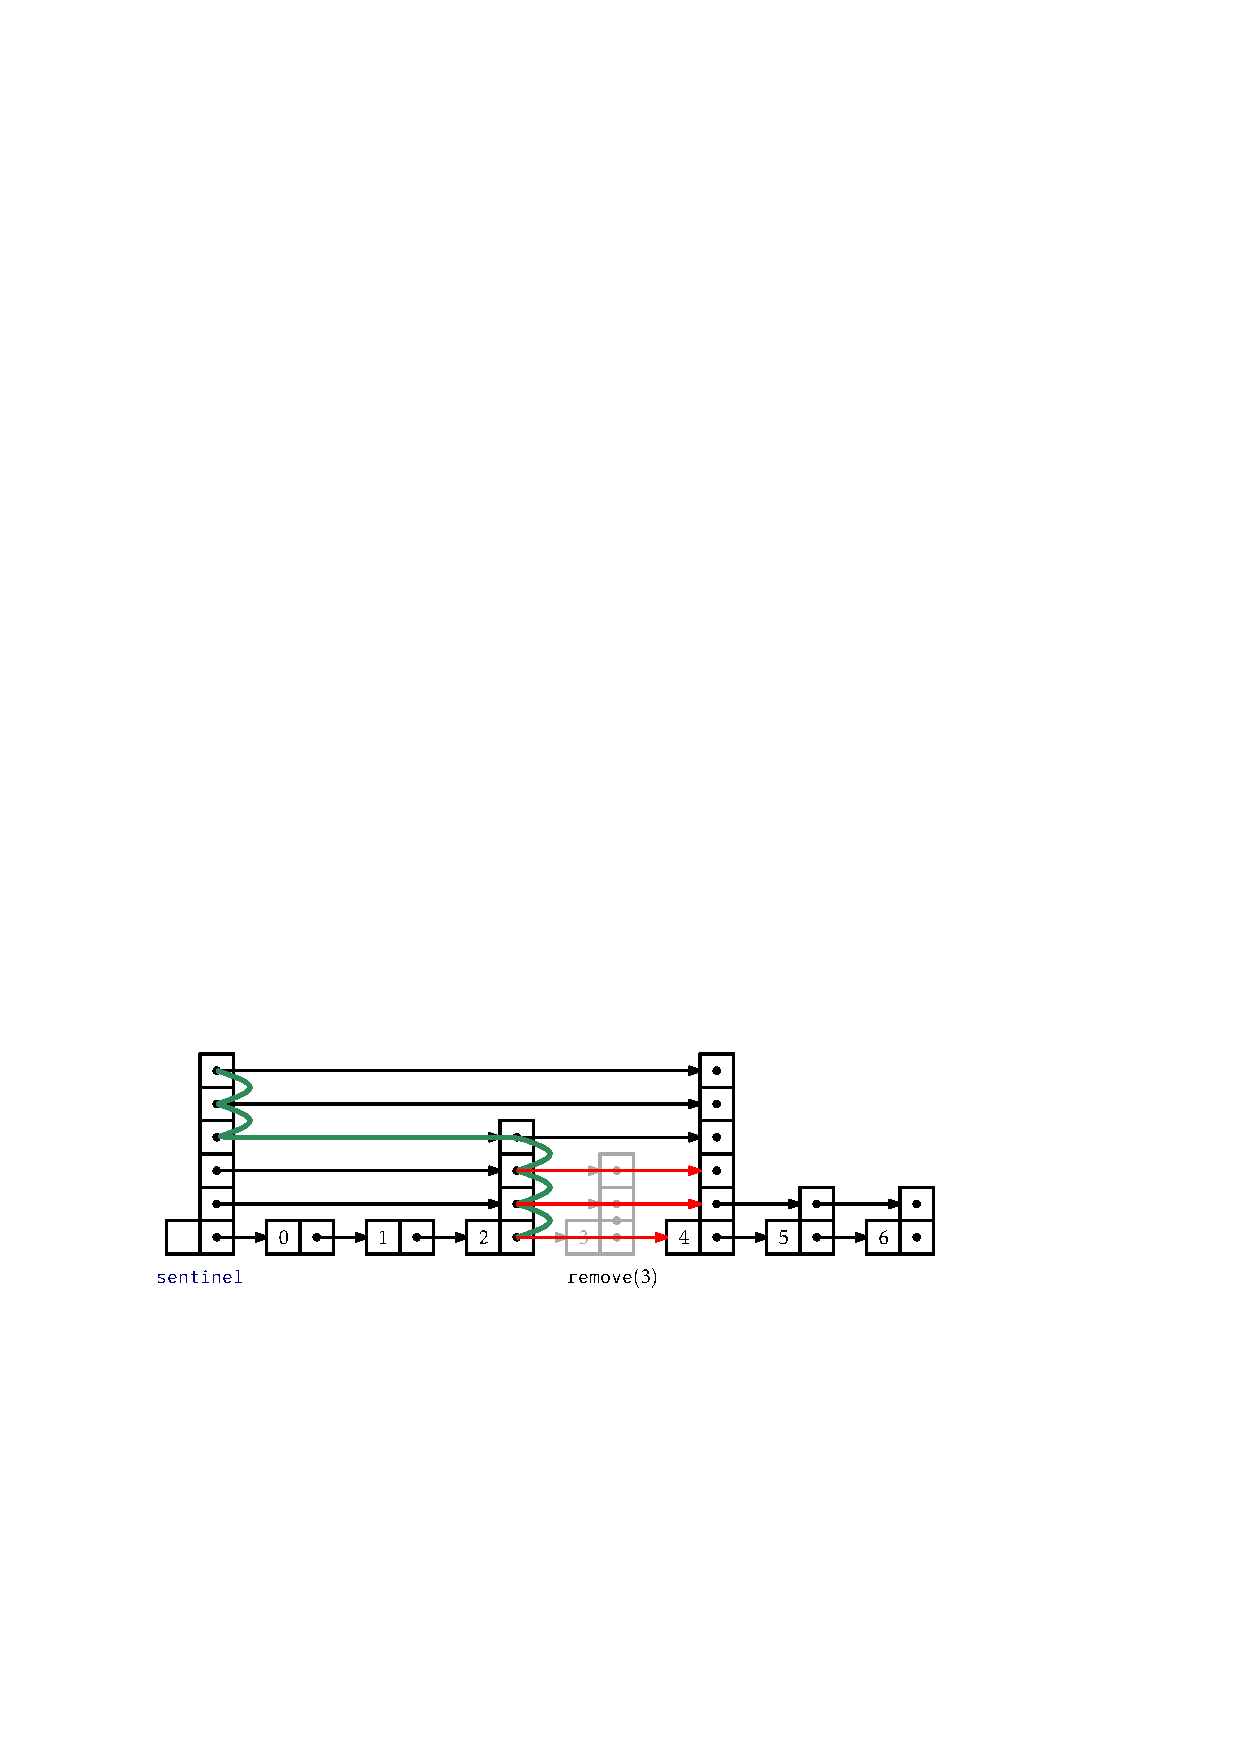
\includegraphics[scale=0.8]{imagens/skiplist-remove}
\end{frame}

\subsection{4.3 SkiplistList}
\begin{frame}
\frametitle{SkiplistList}
Uma SkiplistList implementa um interface de Lista usando uma estrutura de skiplist. Em uma SkiplistList, $L_0$ contém os elementos da lista na ordem em que eles aparecem na lista. Como em uma SkiplistSSet, os elementos podem ser adicionados, removidos e acessados em um tempo $O(\log n)$. 

\end{frame}

\begin{frame}
	\frametitle{SkiplistList}
	Para isto ser possível, precisamos de um meio de acompanhar o caminho de busca para o  $i$-ésimo elemento em $L_0$. O modo mais fácil de fazer isso é definir o conceito de comprimento de uma aresta em uma lista, $L_r$. Definimos o comprimento de cada aresta em  $L_{0}$ como 1. O comprimento da aresta, $e$, em $L_r$, $r>0$, é definido como a soma dos comprimentos das arestas abaixo de $ e$ em $L_{r-1}$. De modo equivalente, o comprimento de $ e$ é o número de arestas em $L_0$ abaixo de $ e$
\end{frame}

\begin{frame}
\frametitle{Comprimento de aresta}
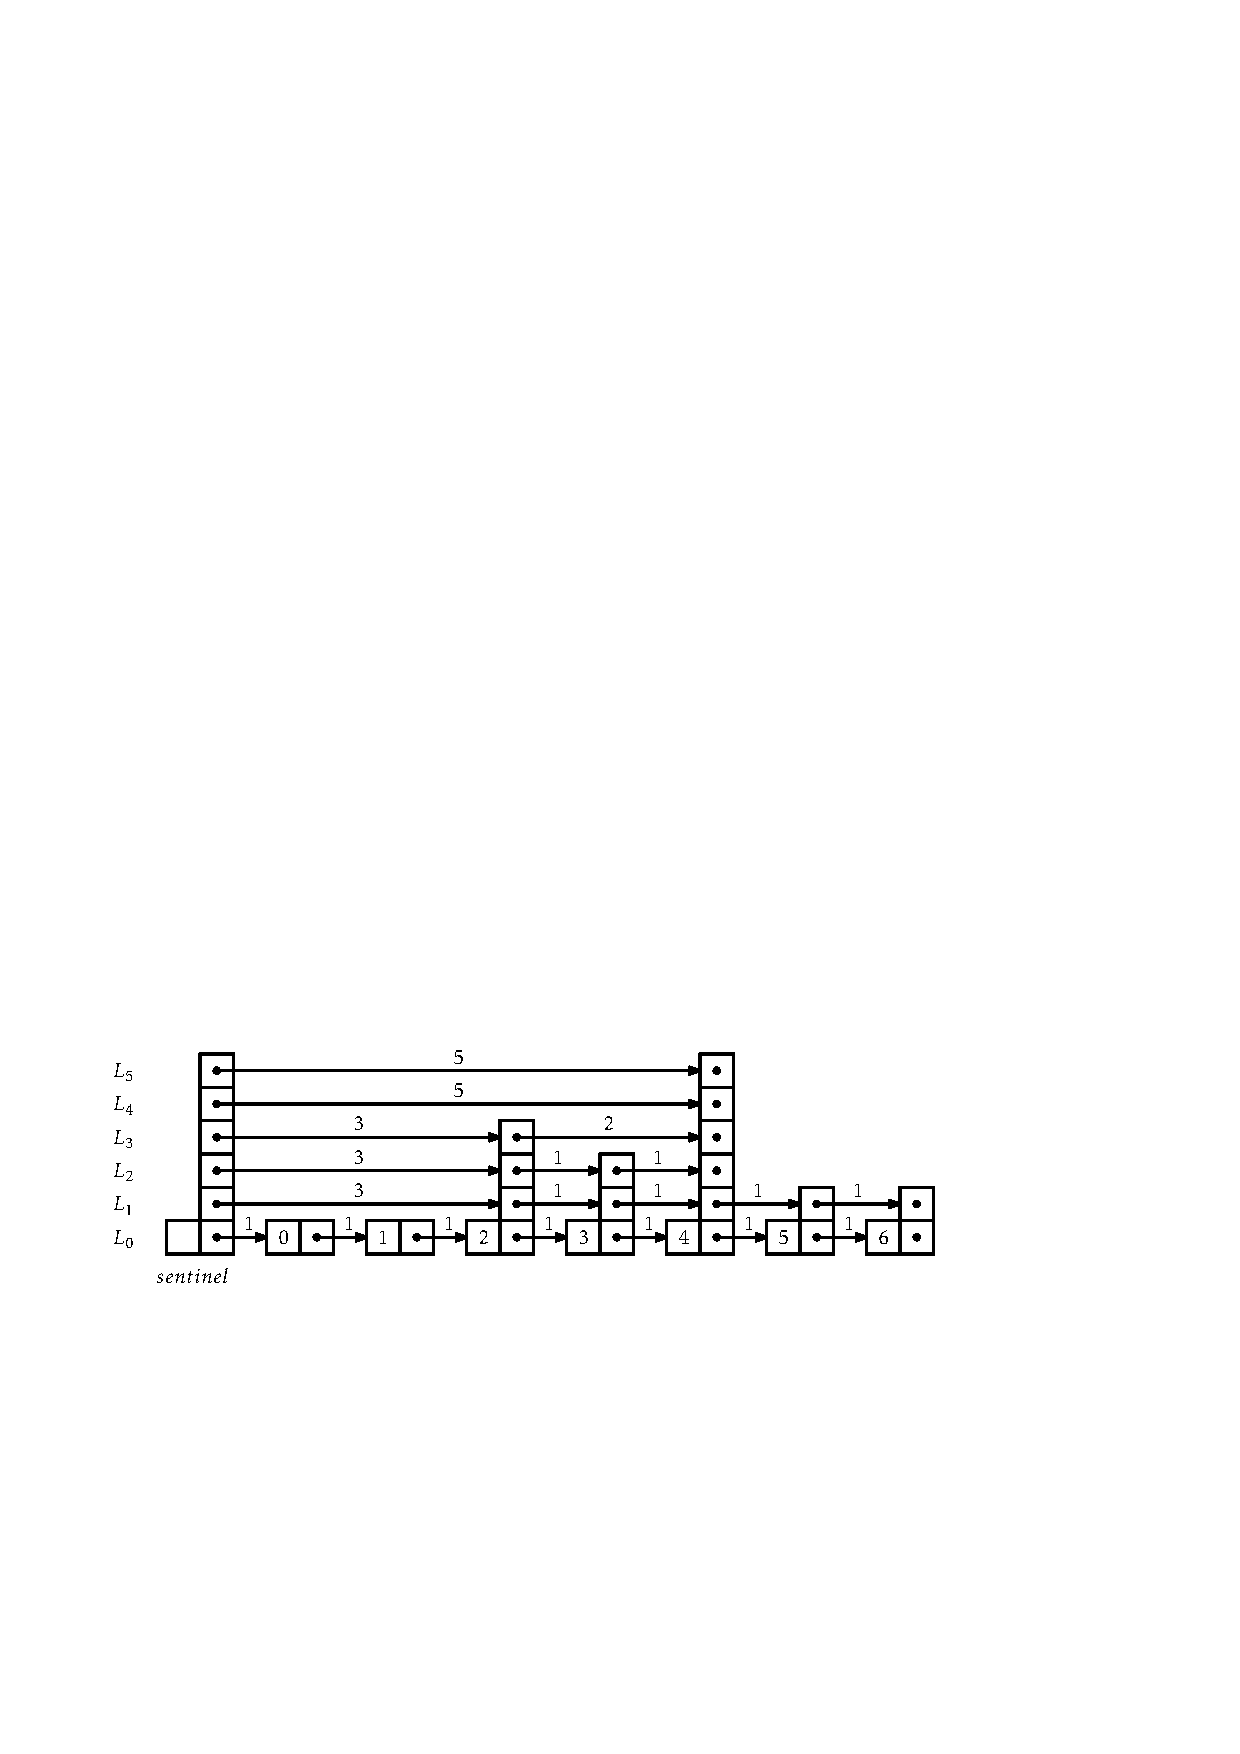
\includegraphics[scale=0.8]{imagens/skiplist-lengths}
\end{frame}

\begin{frame}
\frametitle{$find\_pred(i)$}
\begin{oframed}
\begin{flushleft}
\hspace*{1em} \ensuremath{\mathrm{find\_pred}(\ensuremath{\mathit{i}})}\\
\hspace*{1em} \hspace*{1em} \ensuremath{\ensuremath{\mathit{u}} \gets  \ensuremath{sentinel}}\\
\hspace*{1em} \hspace*{1em} \ensuremath{\ensuremath{\mathit{r}} \gets  \ensuremath{h}}\\
\hspace*{1em} \hspace*{1em} \ensuremath{\ensuremath{\mathit{j}} \gets  \ensuremath{-1}}\\
\hspace*{1em} \hspace*{1em} {\color{black} \textbf{while}} \ensuremath{\ensuremath{\mathit{r}} \ge 0} {\color{black} \textbf{do}} \\
\hspace*{1em} \hspace*{1em} \hspace*{1em} {\color{black} \textbf{while}} \ensuremath{\ensuremath{\mathit{u}}.\ensuremath{\mathit{next}}[\ensuremath{\mathit{r}}] \ne nil} {\color{black} \textbf{and}} \ensuremath{\ensuremath{\mathit{j}} + \ensuremath{\mathit{u}}.\ensuremath{\mathit{length}}[\ensuremath{\mathit{r}}] < i} {\color{black} \textbf{do}} \\
\hspace*{1em} \hspace*{1em} \hspace*{1em} \hspace*{1em} \ensuremath{\ensuremath{\mathit{j}} \gets  \ensuremath{\ensuremath{\mathit{j}} + $u$.\ensuremath{\mathit{length}}[$r$]}}\\
\hspace*{1em} \hspace*{1em} \hspace*{1em} \hspace*{1em} \ensuremath{$u$ \gets  \ensuremath{$u$.\ensuremath{\mathit{next}}[$r$]}  }\ {\color{blue}\# vai para a direita na lista r}\\
\hspace*{1em} \hspace*{1em} \hspace*{1em} \ensuremath{$r$ \gets  \ensuremath{$r$ - 1}  }\ {\color{blue}\# vai para baixo na lista r-1}\\
\hspace*{1em} \hspace*{1em} {\color{black} \textbf{return}} \ensuremath{\ensuremath{\mathit{u}}}\\
\end{flushleft}
\end{oframed}
\end{frame}

\begin{frame}
\frametitle{$get(i)$}
\begin{oframed}
\begin{flushleft}
\hspace*{1em} \ensuremath{\mathrm{get}(\ensuremath{\mathit{i}})}\\

\hspace*{1em} \hspace*{1em} {\color{black} \textbf{return}} \ensuremath{\mathrm{find\_pred}(\ensuremath{\mathit{i}}).\ensuremath{\mathit{next}}[0].\ensuremath{\mathit{x}}}\\
\end{flushleft}
\end{oframed}
\end{frame}

\begin{frame}
\frametitle{$set(i)$}
\begin{oframed}
\begin{flushleft}
\hspace*{1em} \ensuremath{\mathrm{set}(\ensuremath{\mathit{i}}, \ensuremath{\mathit{x}})}\\

\hspace*{1em} \hspace*{1em} \ensuremath{\ensuremath{\mathit{u}} \gets  \ensuremath{\mathrm{find\_pred}(\ensuremath{\mathit{i}}).\ensuremath{\mathit{next}}[0]}}\\
\hspace*{1em} \hspace*{1em} \ensuremath{\ensuremath{\mathit{y}} \gets  \ensuremath{\ensuremath{\mathit{u}}.x}}\\
\hspace*{1em} \hspace*{1em} \ensuremath{\ensuremath{\mathit{u}}.\ensuremath{x} \gets  \ensuremath{x}}\\
\hspace*{1em} \hspace*{1em} {\color{black} \textbf{return}} \ensuremath{\ensuremath{\mathit{y}}}\\
\end{flushleft}
\end{oframed}
\end{frame}



\begin{frame}
\frametitle{$add(4,x)$}
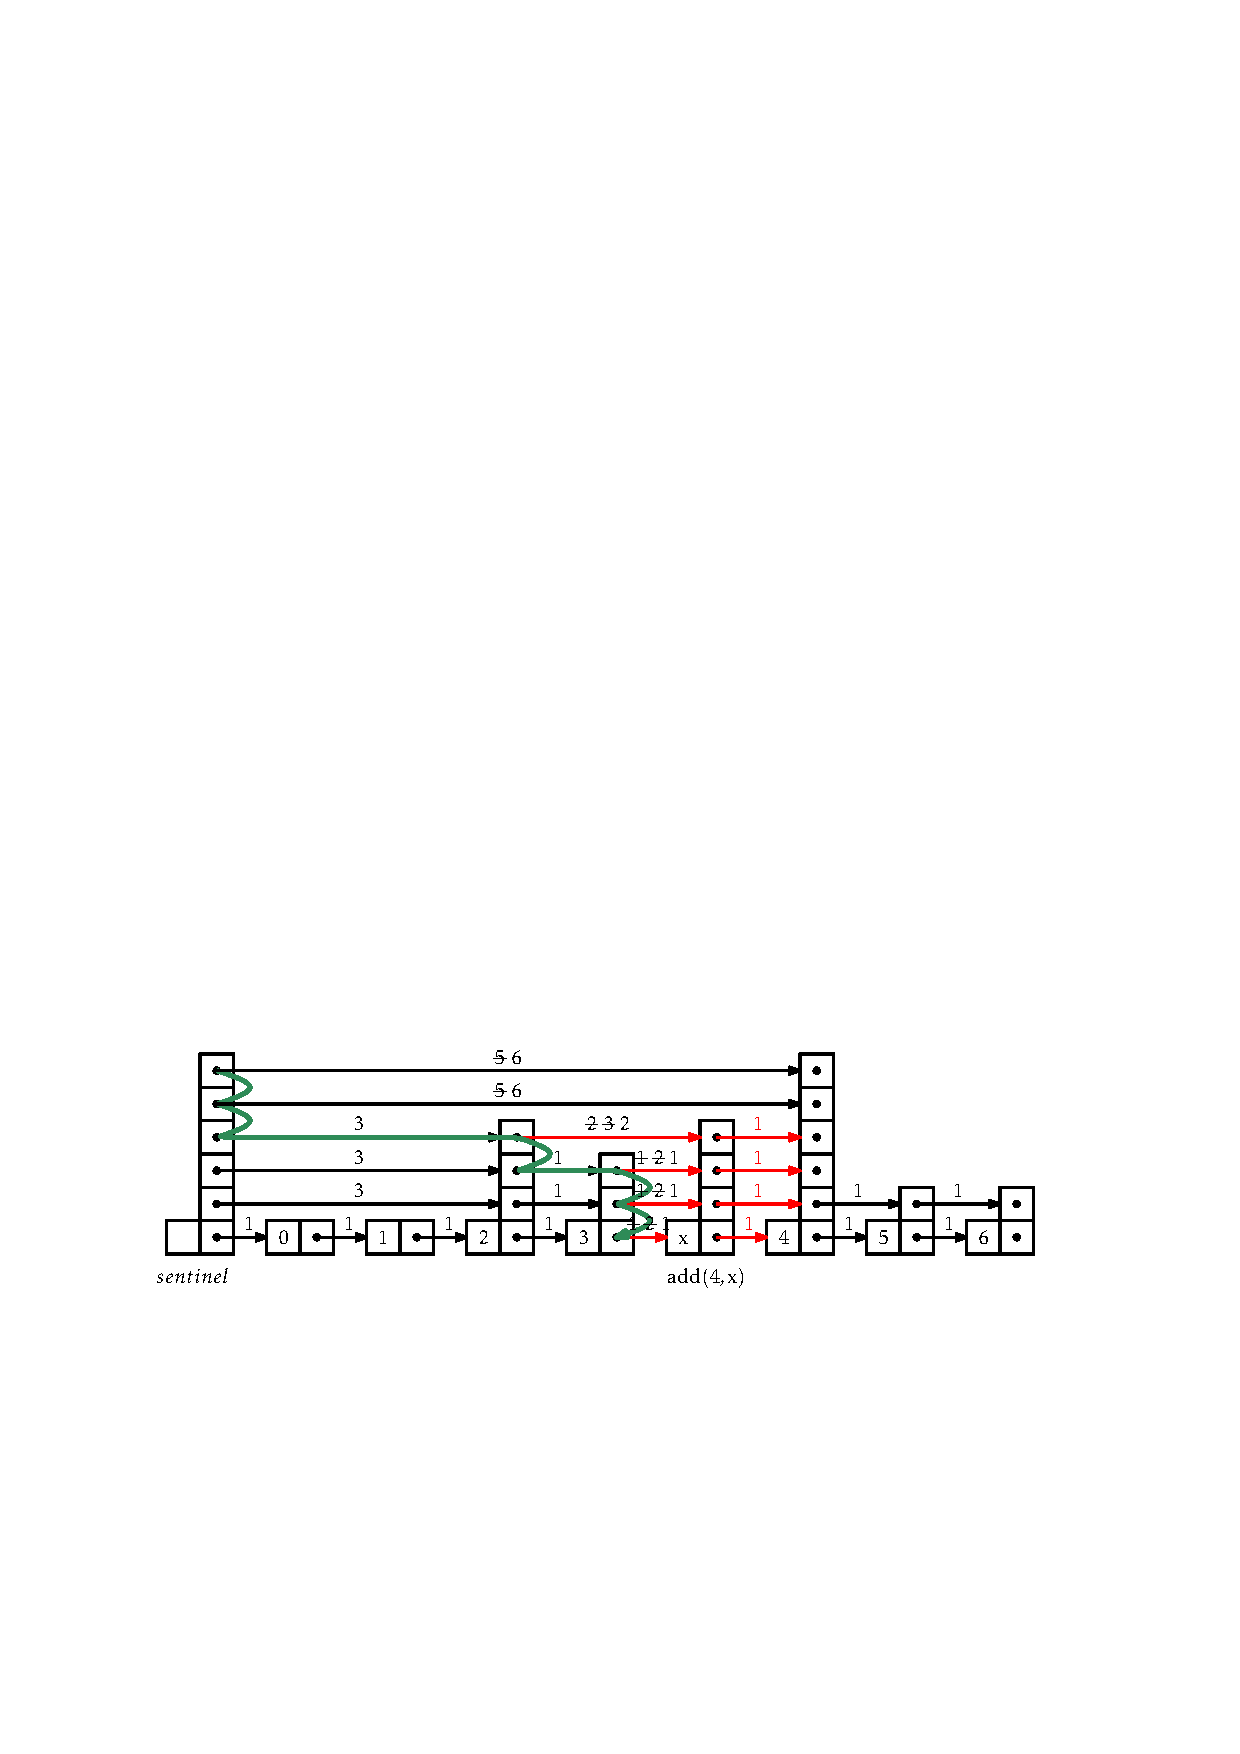
\includegraphics[scale=0.8]{imagens/skiplist-addix}
\end{frame}

\begin{frame}
\frametitle{Atualizando o comprimento das arestas}
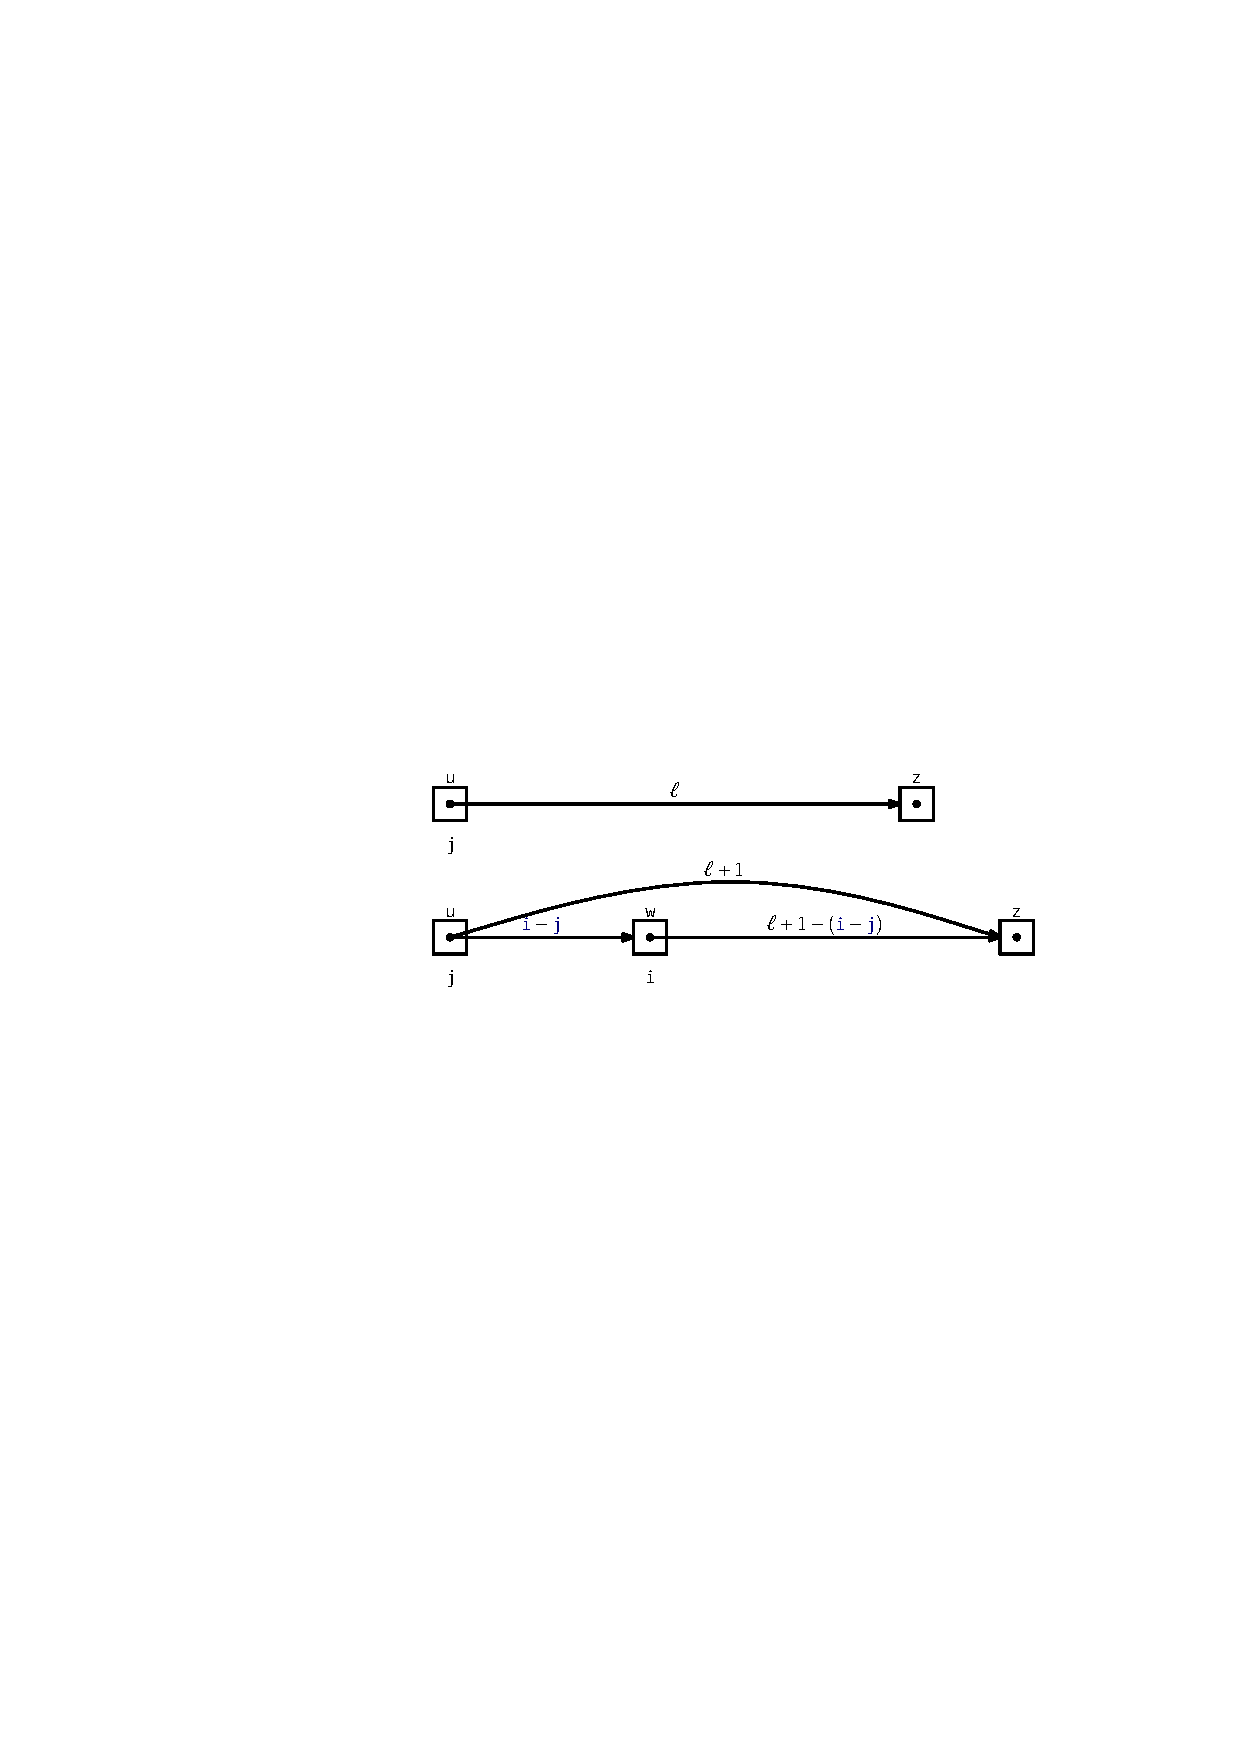
\includegraphics{imagens/skiplist-splice}
\end{frame}

\begin{frame}
\frametitle{$add(i,x)$}
\begin{oframed}
\begin{flushleft}
\hspace*{1em} \ensuremath{\mathrm{add}(\ensuremath{\mathit{i}}, \ensuremath{\mathit{x}})}\\

\hspace*{1em} \hspace*{1em} \ensuremath{\ensuremath{\mathit{w}} \gets  \ensuremath{\mathrm{new\_node}(\ensuremath{\mathit{x}}, \mathrm{pick\_height}()})}\\
\hspace*{1em} \hspace*{1em} {\color{black} \textbf{if}} \ensuremath{\ensuremath{\mathit{w}}.\mathrm{height}() > h} {\color{black} \textbf{then}} \\
\hspace*{1em} \hspace*{1em} \hspace*{1em} \ensuremath{\ensuremath{\mathit{h}} \gets  \ensuremath{\ensuremath{\mathit{w}}.\mathrm{height}()}}\\
\hspace*{1em} \hspace*{1em} \ensuremath{\mathrm{add}(\ensuremath{\mathit{i}}, \ensuremath{\mathit{w}})}\\
\end{flushleft}
\end{oframed}
\end{frame}

\begin{frame}[shrink]
\frametitle{$add(i,w)$}
\begin{oframed}
\begin{flushleft}
\hspace*{1em} \ensuremath{\mathrm{add}(\ensuremath{\mathit{i}}, \ensuremath{\mathit{w}})}\\
\hspace*{1em} \hspace*{1em} \ensuremath{\ensuremath{\mathit{u}} \gets  \ensuremath{sentinel}}\\
\hspace*{1em} \hspace*{1em} \ensuremath{\ensuremath{\mathit{k}} \gets  \ensuremath{\ensuremath{\mathit{w}}.\mathrm{height}()}}\\
\hspace*{1em} \hspace*{1em} \ensuremath{\ensuremath{\mathit{r}} \gets  \ensuremath{h}}\\
\hspace*{1em} \hspace*{1em} \ensuremath{\ensuremath{\mathit{j}} \gets  \ensuremath{-1}}\\
\hspace*{1em} \hspace*{1em} {\color{black} \textbf{while}} \ensuremath{\ensuremath{\mathit{r}} \ge 0} {\color{black} \textbf{do}} \\
\hspace*{1em} \hspace*{1em} \hspace*{1em} {\color{black} \textbf{while}} \ensuremath{\ensuremath{\mathit{u}}.\ensuremath{\mathit{next}}[\ensuremath{\mathit{r}}] \ne nil} {\color{black} \textbf{and}} \ensuremath{\ensuremath{\mathit{j}}+\ensuremath{\mathit{u}}.\ensuremath{\mathit{length}}[\ensuremath{\mathit{r}}] < i} {\color{black} \textbf{do}} \\
\hspace*{1em} \hspace*{1em} \hspace*{1em} \hspace*{1em} \ensuremath{\ensuremath{\mathit{j}} \gets  \ensuremath{\ensuremath{\mathit{j}} + \ensuremath{\mathit{u}}.\ensuremath{\mathit{length}}[\ensuremath{\mathit{r}}]}}\\
\hspace*{1em} \hspace*{1em} \hspace*{1em} \hspace*{1em} \ensuremath{\ensuremath{\mathit{u}} \gets  \ensuremath{\ensuremath{\mathit{u}}.\ensuremath{\mathit{next}}[\ensuremath{\mathit{r}}]}}\\
\hspace*{1em} \hspace*{1em} \hspace*{1em} \ensuremath{\ensuremath{\mathit{u}}.\ensuremath{\ensuremath{\mathit{length}}[\ensuremath{\mathit{r}}]} \gets  \ensuremath{\ensuremath{\mathit{u}}.\ensuremath{\mathit{length}}[\ensuremath{\mathit{r}}] + 1}}\\
\hspace*{1em} \hspace*{1em} \hspace*{1em} {\color{black} \textbf{if}} \ensuremath{\ensuremath{\mathit{r}} \le k} {\color{black} \textbf{then}} \\
\hspace*{1em} \hspace*{1em} \hspace*{1em} \hspace*{1em} \ensuremath{\ensuremath{\mathit{w}}.\ensuremath{\ensuremath{\mathit{next}}[\ensuremath{\mathit{r}}]} \gets  \ensuremath{\ensuremath{\mathit{u}}.\ensuremath{\mathit{next}}[\ensuremath{\mathit{r}}]}}\\
\hspace*{1em} \hspace*{1em} \hspace*{1em} \hspace*{1em} \ensuremath{\ensuremath{\mathit{u}}.\ensuremath{\ensuremath{\mathit{next}}[\ensuremath{\mathit{r}}]} \gets  \ensuremath{w}}\\
\hspace*{1em} \hspace*{1em} \hspace*{1em} \hspace*{1em} \ensuremath{\ensuremath{\mathit{w}}.\ensuremath{\ensuremath{\mathit{length}}[\ensuremath{\mathit{r}}]} \gets  \ensuremath{\ensuremath{\mathit{u}}.\ensuremath{\mathit{length}}[\ensuremath{\mathit{r}}] - (\ensuremath{\mathit{i}}-\ensuremath{\mathit{j}})}}\\
\hspace*{1em} \hspace*{1em} \hspace*{1em} \hspace*{1em} \ensuremath{\ensuremath{\mathit{u}}.\ensuremath{\ensuremath{\mathit{length}}[\ensuremath{\mathit{r}}]} \gets  \ensuremath{\ensuremath{\mathit{i}} - j}}\\
\hspace*{1em} \hspace*{1em} \hspace*{1em} \ensuremath{\ensuremath{\mathit{r}} \gets  \ensuremath{\ensuremath{\mathit{r}} - 1}}\\
\hspace*{1em} \hspace*{1em} \ensuremath{\ensuremath{\mathit{n}} \gets  \ensuremath{\ensuremath{\mathit{n}} + 1}}\\
\hspace*{1em} \hspace*{1em} {\color{black} \textbf{return}} \ensuremath{\ensuremath{\mathit{u}}}\\
\end{flushleft}
\end{oframed}
\end{frame}

\begin{frame}
\frametitle{$remove(3)$}
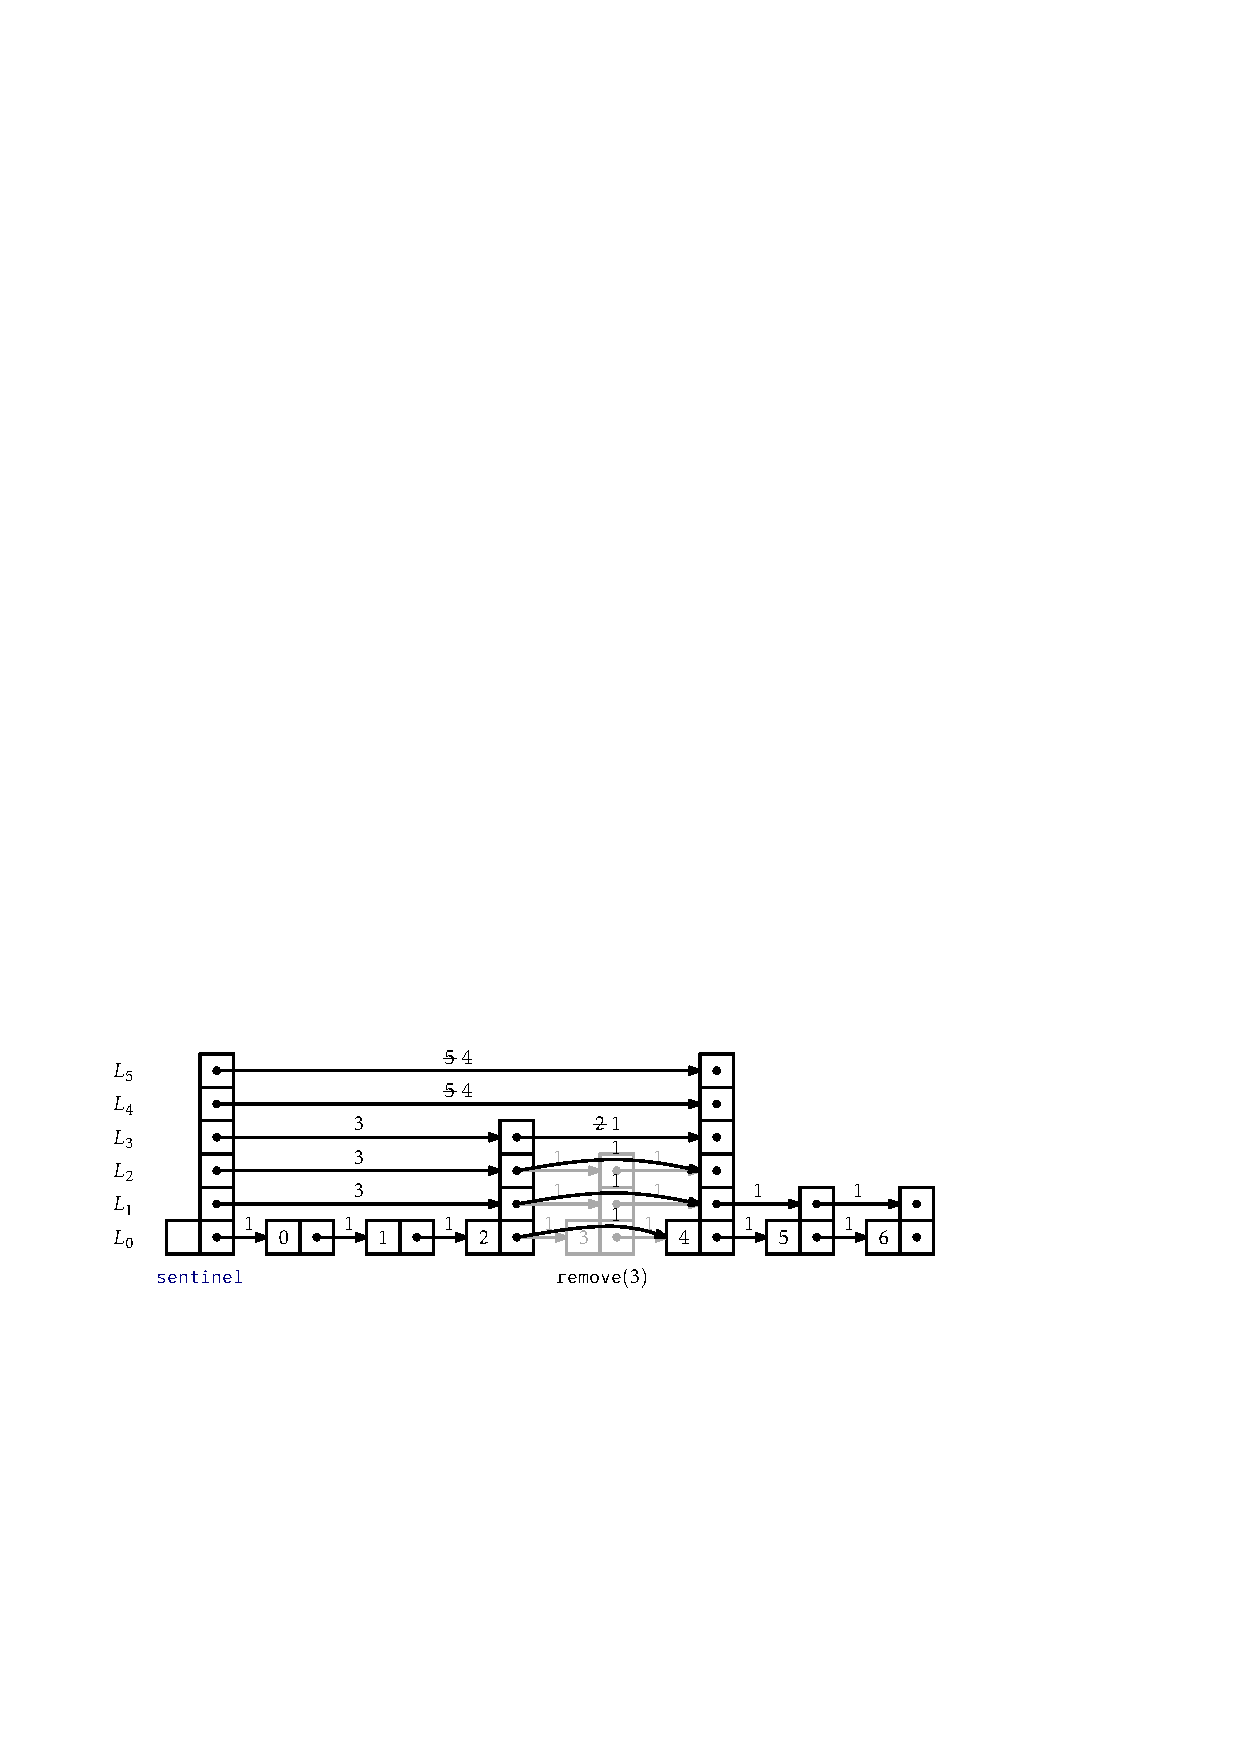
\includegraphics[scale=0.8]{imagens/skiplist-removei}
\end{frame}


\begin{frame}[shrink]
\frametitle{$remove(i)$}
\begin{oframed}
\begin{flushleft}
\hspace*{1em} \ensuremath{\mathrm{remove}(\ensuremath{\mathit{i}})}\\

\hspace*{1em} \hspace*{1em} \ensuremath{\ensuremath{\mathit{u}} \gets  \ensuremath{sentinel}}\\
\hspace*{1em} \hspace*{1em} \ensuremath{\ensuremath{\mathit{r}} \gets  \ensuremath{h}}\\
\hspace*{1em} \hspace*{1em} \ensuremath{\ensuremath{\mathit{j}} \gets  \ensuremath{-1}}\\
\hspace*{1em} \hspace*{1em} {\color{black} \textbf{while}} \ensuremath{\ensuremath{\mathit{r}} \ge 0} {\color{black} \textbf{do}} \\
\hspace*{1em} \hspace*{1em} \hspace*{1em} {\color{black} \textbf{while}} \ensuremath{\ensuremath{\mathit{u}}.\ensuremath{\mathit{next}}[\ensuremath{\mathit{r}}] \ne nil} {\color{black} \textbf{and}} \ensuremath{\ensuremath{\mathit{j}} + \ensuremath{\mathit{u}}.\ensuremath{\mathit{length}}[\ensuremath{\mathit{r}}] < i} {\color{black} \textbf{do}} \\
\hspace*{1em} \hspace*{1em} \hspace*{1em} \hspace*{1em} \ensuremath{\ensuremath{\mathit{j}} \gets  \ensuremath{\ensuremath{\mathit{j}} + \ensuremath{\mathit{u}}.\ensuremath{\mathit{length}}[\ensuremath{\mathit{r}}]}}\\
\hspace*{1em} \hspace*{1em} \hspace*{1em} \hspace*{1em} \ensuremath{\ensuremath{\mathit{u}} \gets  \ensuremath{\ensuremath{\mathit{u}}.\ensuremath{\mathit{next}}[\ensuremath{\mathit{r}}]}}\\
\hspace*{1em} \hspace*{1em} \hspace*{1em} \ensuremath{\ensuremath{\mathit{u}}.\ensuremath{\ensuremath{\mathit{length}}[\ensuremath{\mathit{r}}]} \gets  \ensuremath{\ensuremath{\mathit{u}}.\ensuremath{\mathit{length}}[\ensuremath{\mathit{r}}] - 1}}\\
\hspace*{1em} \hspace*{1em} \hspace*{1em} {\color{black} \textbf{if}} \ensuremath{\ensuremath{\mathit{j}} + \ensuremath{\mathit{u}}.\ensuremath{\mathit{length}}[\ensuremath{\mathit{r}}] + 1 \eq i} {\color{black} \textbf{and}} \ensuremath{\ensuremath{\mathit{u}}.\ensuremath{\mathit{next}}[\ensuremath{\mathit{r}}] \ne nil} {\color{black} \textbf{then}} \\
\hspace*{1em} \hspace*{1em} \hspace*{1em} \hspace*{1em} \ensuremath{\ensuremath{\mathit{x}} \gets  \ensuremath{\ensuremath{\mathit{u}}.\ensuremath{\mathit{next}}[\ensuremath{\mathit{r}}].x}}\\
\hspace*{1em} \hspace*{1em} \hspace*{1em} \hspace*{1em} \ensuremath{\ensuremath{\mathit{u}}.\ensuremath{\ensuremath{\mathit{length}}[\ensuremath{\mathit{r}}]} \gets  \ensuremath{\ensuremath{\mathit{u}}.\ensuremath{\mathit{length}}[\ensuremath{\mathit{r}}] + \ensuremath{\mathit{u}}.\ensuremath{\mathit{next}}[\ensuremath{\mathit{r}}].\ensuremath{\mathit{length}}[\ensuremath{\mathit{r}}]}}\\
\hspace*{1em} \hspace*{1em} \hspace*{1em} \hspace*{1em} \ensuremath{\ensuremath{\mathit{u}}.\ensuremath{\ensuremath{\mathit{next}}[\ensuremath{\mathit{r}}]} \gets  \ensuremath{\ensuremath{\mathit{u}}.\ensuremath{\mathit{next}}[\ensuremath{\mathit{r}}].\ensuremath{\mathit{next}}[\ensuremath{\mathit{r}}]}}\\
\hspace*{1em} \hspace*{1em} \hspace*{1em} \hspace*{1em} {\color{black} \textbf{if}} \ensuremath{\ensuremath{\mathit{u}} \eq sentinel} {\color{black} \textbf{and}} \ensuremath{\ensuremath{\mathit{u}}.\ensuremath{\mathit{next}}[\ensuremath{\mathit{r}}] \eq nil} {\color{black} \textbf{then}} \\
\hspace*{1em} \hspace*{1em} \hspace*{1em} \hspace*{1em} \hspace*{1em} \ensuremath{\ensuremath{\mathit{h}} \gets  \ensuremath{\ensuremath{\mathit{h}} - 1}}\\
\hspace*{1em} \hspace*{1em} \hspace*{1em} \ensuremath{\ensuremath{\mathit{r}} \gets  \ensuremath{\ensuremath{\mathit{r}} - 1}}\\
\hspace*{1em} \hspace*{1em} \ensuremath{\ensuremath{\mathit{n}} \gets  \ensuremath{\ensuremath{\mathit{n}} - 1}}\\
\hspace*{1em} \hspace*{1em} {\color{black} \textbf{return}} \ensuremath{x}\hspace*{1em} \\
\end{flushleft}
\end{oframed}
\end{frame}


\begin{frame}
FIM
\end{frame}
\end{document}
